\documentclass{article}
\usepackage{xeCJK,amsmath,geometry,graphicx,amssymb,zhnumber,booktabs,setspace,tasks,verbatim,amsthm,amsfonts,mathdots}
\usepackage{listings,xcolor}
\geometry{a4paper,scale=0.8}   
\title{ICS  HomeWork-1}
\author{PB20000113孔浩宇}
\begin{document}
\maketitle
\section*{T1}如图
\begin{figure}[h]
    \centering
    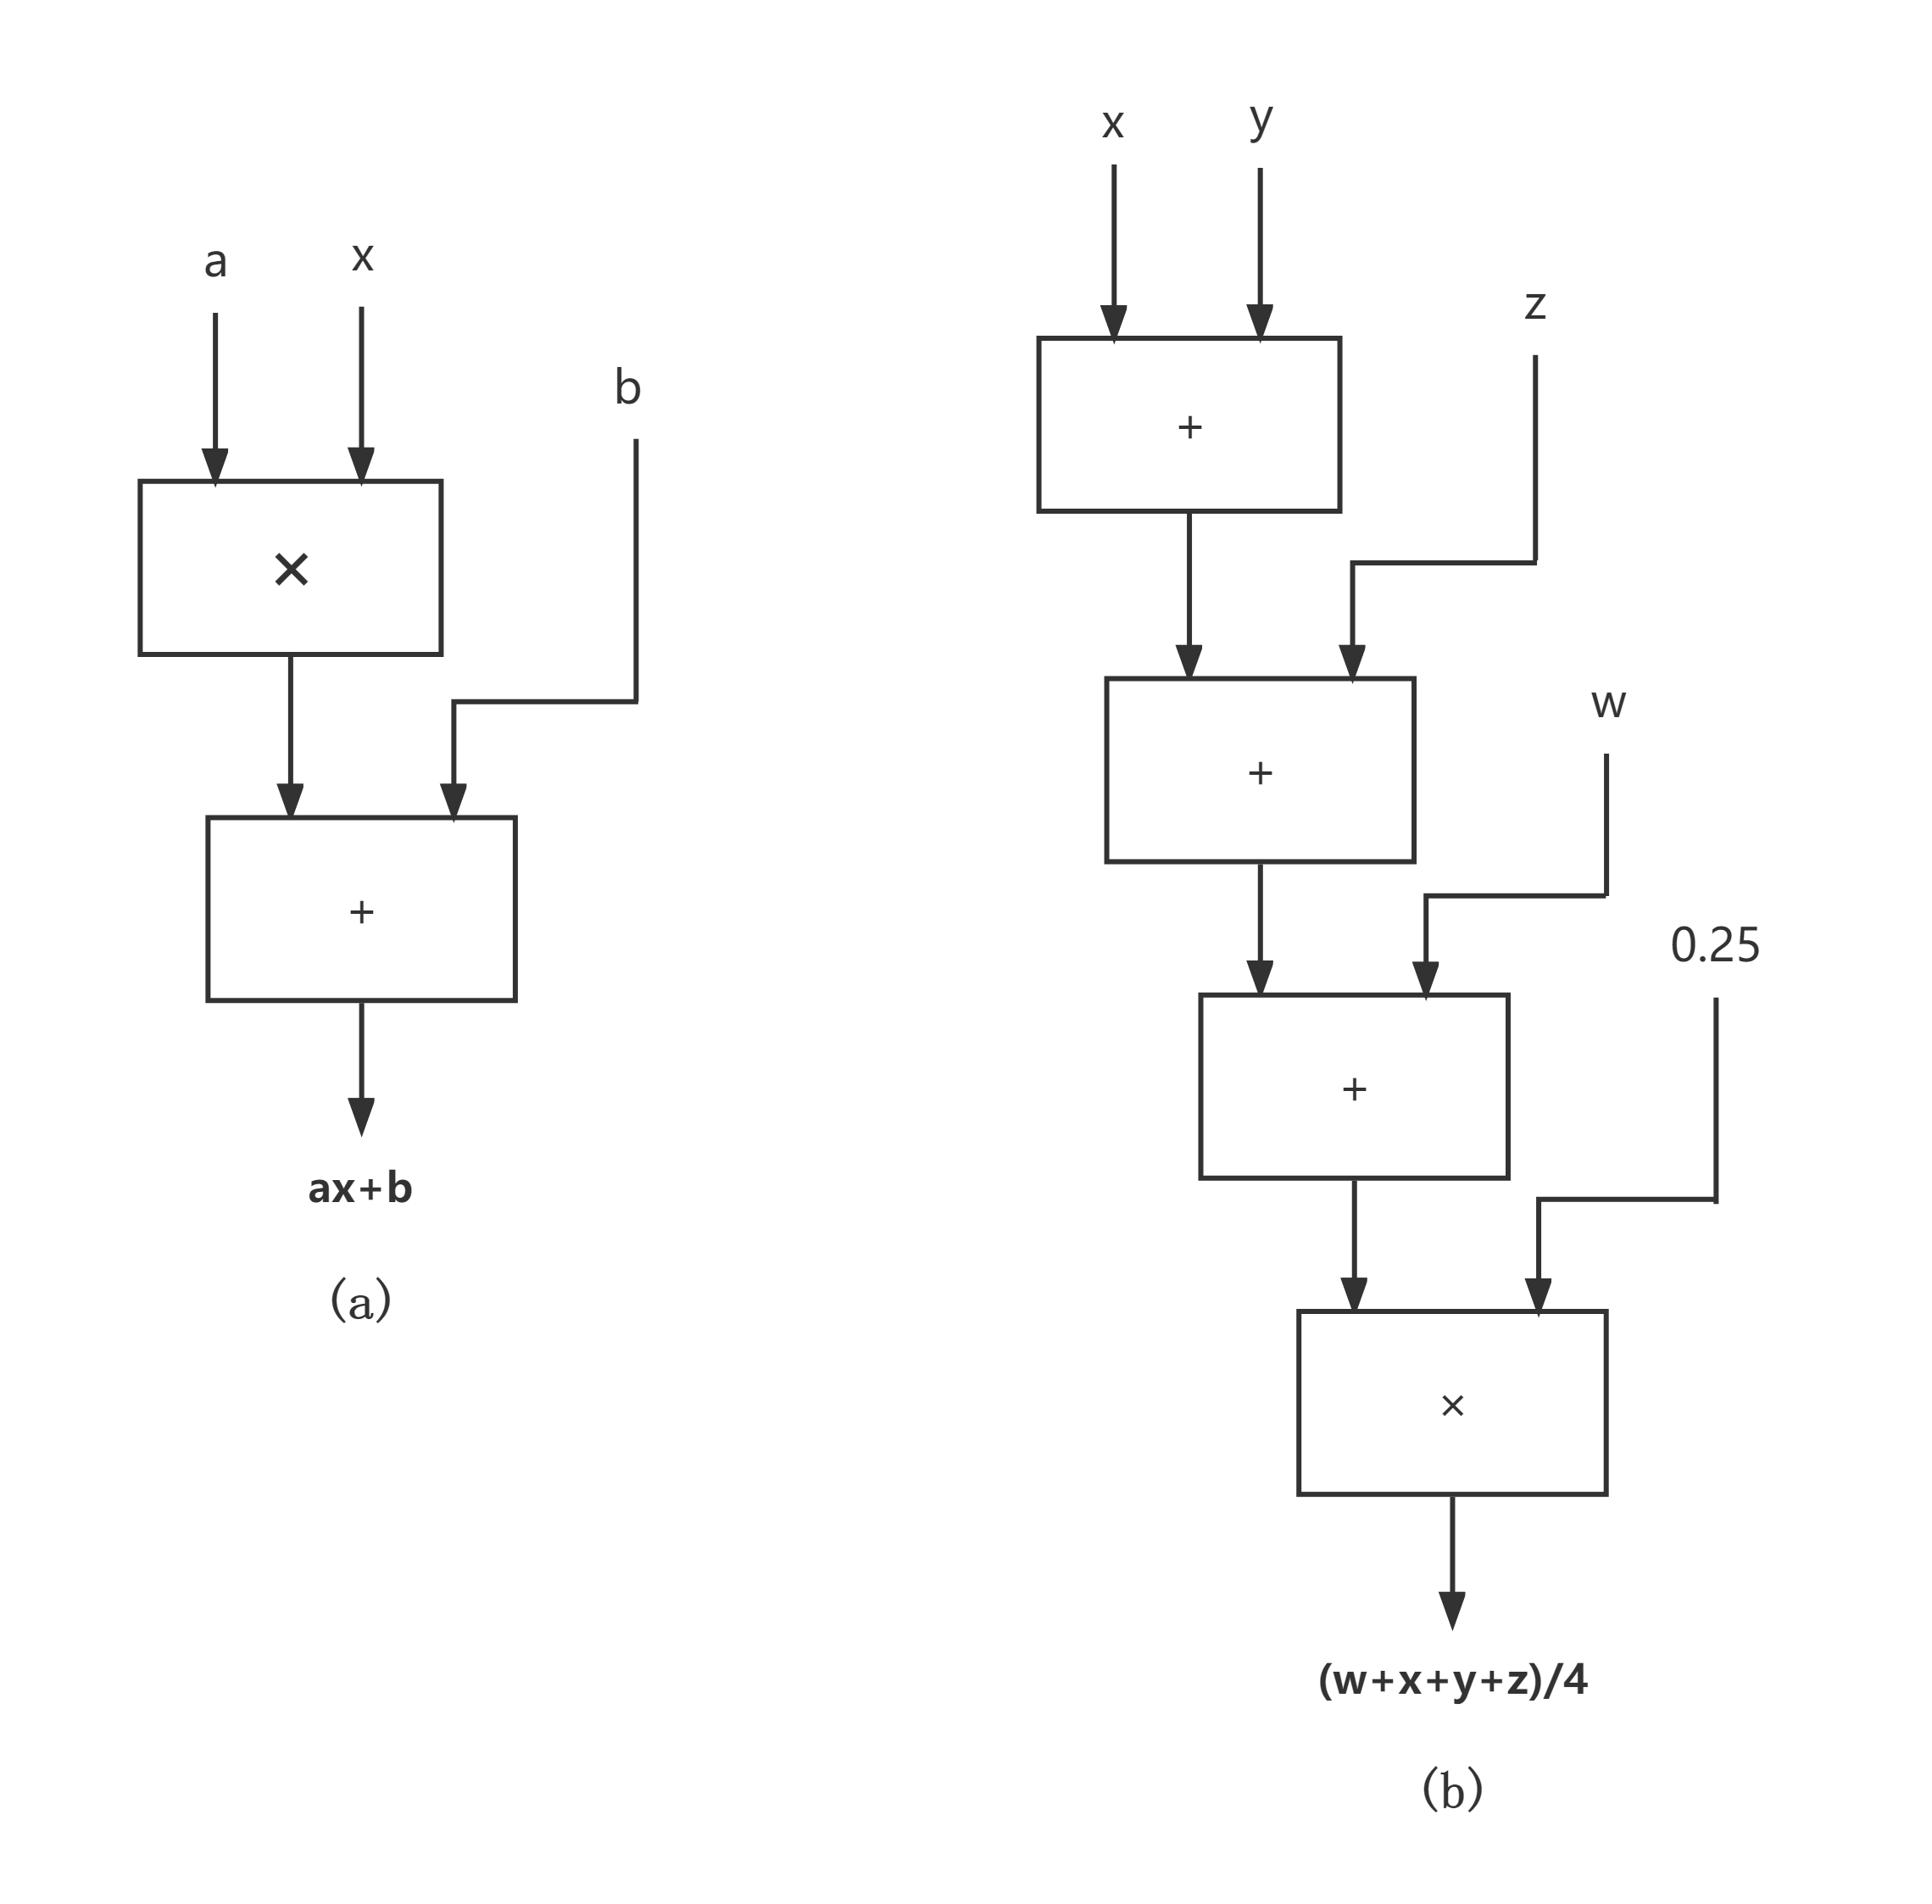
\includegraphics[scale=0.2]{01.png}
\end{figure}
\clearpage
\begin{figure}[h]
    \centering
    \includegraphics*[scale=0.25]{02.png}
\end{figure}
\begin{figure}[h]
    \centering
    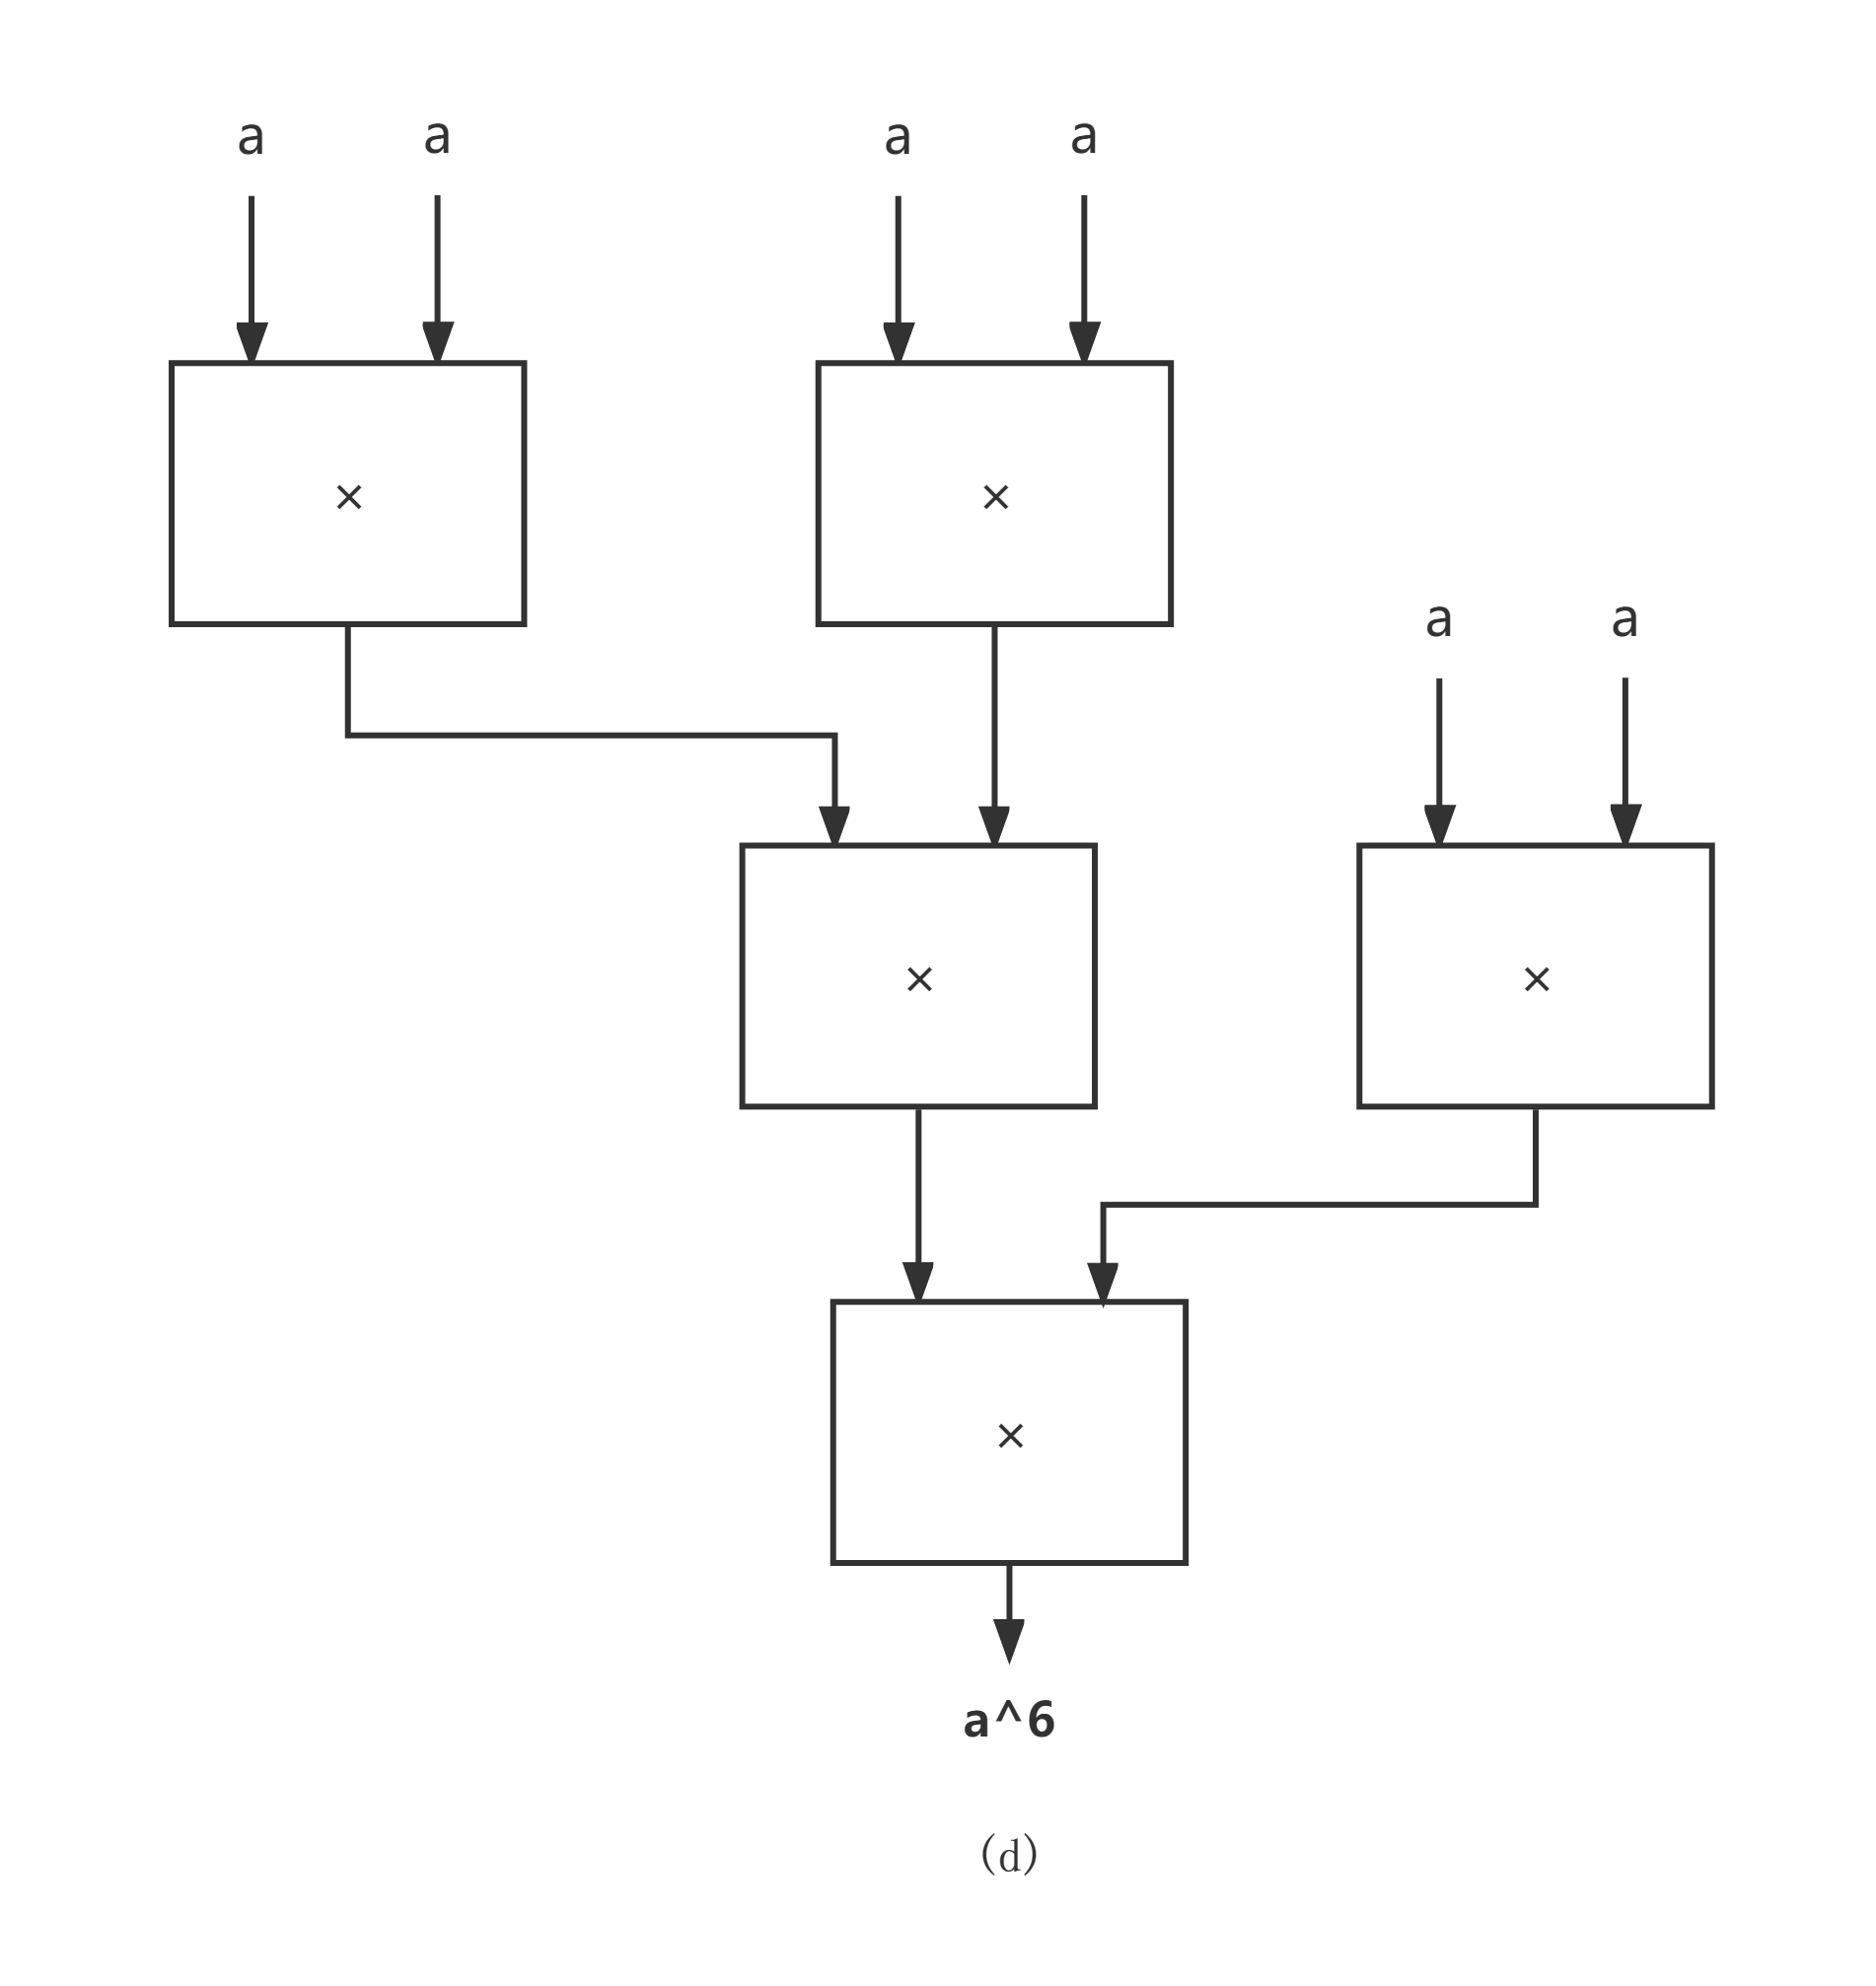
\includegraphics[scale=0.25]{03.png}
\end{figure}
\clearpage
\section*{T2}
    \subsection*{a.}
        \[
            {(98)}_D={(01100010)}_B
            \Rightarrow\ 
            {(98)}_{\mbox{补}}=01100010.
        \]    
    \subsection*{b.}
        \[
            {(-105)}_D={(11101001)}_B
            \Rightarrow\ 
            {(-105)}_{\mbox{补}}=00010111.
        \]
    \subsection*{c.}
        \[
            01000010(\mbox{补})=01000010\mbox{原}={(66)}_D.
        \]
    \subsection*{d.}
        \[
            11101111(\mbox{补})=10010001\mbox{原}={(-17)}_D.  
        \]
\section*{T3}
    \subsection*{a.}
        \begin{align*}
            {(01)}_{\mbox{补}}+{(110011)}_{\mbox{补}}
            =&{(000001)}_{\mbox{补}}+{(110011)}_{\mbox{补}}\\
            =&{(110100)}_{\mbox{补}}\\
            =&{(101100)}_{\mbox{原}}\\
            =&{(-12)}_D.
        \end{align*}
    \subsection*{b.}
        \begin{align*}
            {(111)}_{\mbox{补}}+{(0100110)}_{\mbox{补}}
            =&{(1111111)}_{\mbox{补}}+{(0100110)}_{\mbox{补}}\\
            =&{(0100101)}_{\mbox{补}}\\
            =&{(0100101)}_{\mbox{补}}\\
            =&{(37)}_D.
        \end{align*}
    \subsection*{c.}
        \begin{align*}
            {(1010)}_{\mbox{补}}+{(1101)}_{\mbox{补}}
            =&{(0111)}_{\mbox{补}}\\
            =&{(7)}_D.\ (\mbox{溢出})
        \end{align*}
    \subsection*{d.}
\section*{T4}
    \subsection*{a.}
        \[
            {(101011)}_{\mbox{补}}={(11101011)}_{\mbox{补}}.
        \]
    \subsection*{b.}
        \[
            {(011110)}_{\mbox{补}}={(00011110)}_{\mbox{补}}.
        \]
    \subsection*{c.}
        \[
            {(11111111110000)}_{\mbox{补}}={(11110000)}_{\mbox{补}}.
        \]
    \subsection*{d.}
        \[
            {(00001)}_{\mbox{补}}={(00000001)}_{\mbox{补}}.
        \]
\section*{T5}
    \begin{align*}
        4.3(D)
        =&100.0100 1100 1100 1100 11001(B) \ (\mbox{取小数点后21位})\\
        =&{(-1)}^{0}\times 1.000100110011\times 2^{2}\\
        \xrightarrow{IEEE754}& 0\ 1000 0001\ 0001 0011 0011 0011 0011 001.
    \end{align*}
\section*{T6}
    \begin{align*}
        0\ 1000 1001\ 1111 1001 1010 0100 0000 000
        &=1 1111 1001 10.1001 0000 0000 0(B)\\
        &=2022.5625(D).
    \end{align*}
\section*{T7}
    \begin{enumerate}
        \item [(1)]
        \begin{enumerate}
            \item [a.]
            \[
                10100101\ \mbox{AND}\ 11010101= 10000101.
            \]
            \item [b.]
            \[
                10001110\ \mbox{OR}\ 11110101=1111 1111.
            \]
            \item [c.]
            \[
                \mbox{NOT}(11110001)=00001110.
            \]
        \end{enumerate}
        \item [(2)]
        \begin{enumerate}
            \item [d.]
            \begin{align*}
                &(\mbox{x}1234\ \mbox{AND}\ \mbox{x}5678)\ \mbox{OR}\ (\mbox{x}ABCD\ \mbox{AND}\ \mbox{x}99EF)\\
                =&(0001 0010 0011 0100\ \mbox{AND}\ 0101 0110 0111 1000)\ \mbox{OR}\ (1010 1011 1100 1101\ \mbox{AND}\ 1001 1001 1110 1111)\\
                =&(0001 0010 0011 0000)\ \mbox{OR}\ (1000 1001 1100 1101)\\
                =& 1001 1011 1111 1101\\
                =& \mbox{x}9BFD.
            \end{align*}
            \item [e.]
            \begin{align*}
                \mbox{x}6A12\ \mbox{XOR}\ \mbox{x}3A15
                &=0110 1010 0001 0010\ \mbox{XOR}\ 0011 1010 0001 0101\\
                &=0101 0000 0000 0111\\
                &=\mbox{x}5007.
            \end{align*}
        \end{enumerate}
    \end{enumerate}
\clearpage
\section*{T8}如图,$Q_2=A\ \mbox{AND}\ B\ \mbox{AND}\ C.$
\begin{figure}[h]
    \centering
    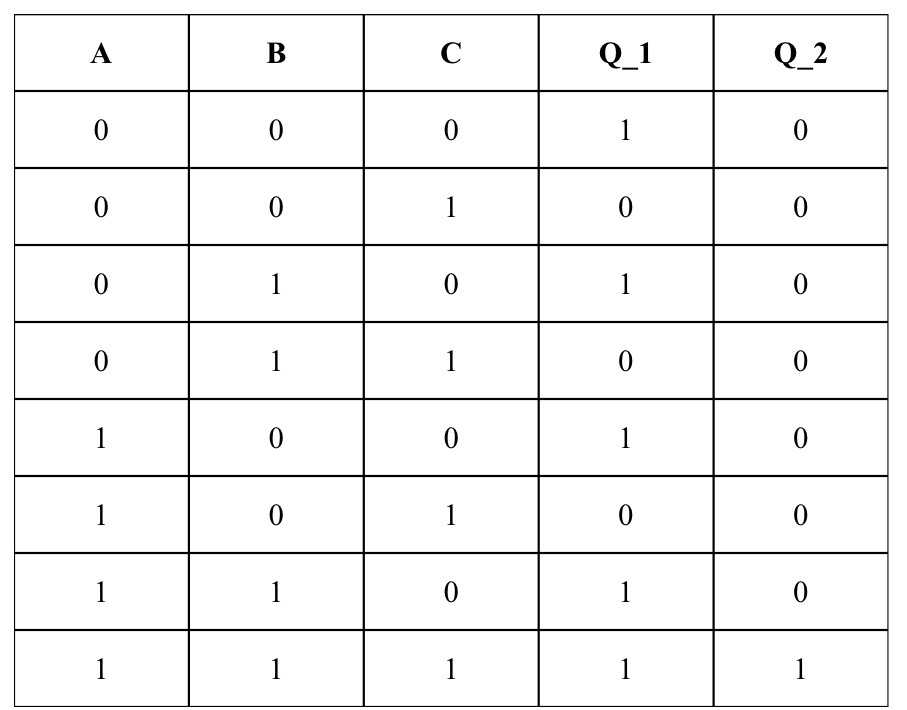
\includegraphics[scale=0.5]{04.jpg}
\end{figure}
\section*{T9}
\begin{enumerate}
    \item [(1)]
    \[
        '\backslash t \backslash n \backslash r'=00001001 00001010 00001101=CQoN.
    \]
    \item [(2)]
    在MIME格式的电子邮件中,base64可以用来将binary的字节序列数据编码成ASCII字符序列构成的文本。
    使用时,在传输编码方式中指定base64。使用的字符包括大小写字母各26个,
    加上10个数字,和加号“+”,斜杠“$\backslash$”,一共64个字符,等号“=”用来作为后缀用途。
\end{enumerate}
\section*{T10}
    \begin{align*}
        \mbox{MAX}
        =&{(-1)}^0\times 1.1111 1111 1111 1111 1111 111\times 2^{254-127}\\
        =&1.1111 1111 1111 1111 1111 111\times 2^{127}.
    \end{align*}
\clearpage
\section*{T11}如图,$C=\left\{ \{ 0,M \},E[24:47]\right\}$.
\begin{figure}[h]
    \centering
    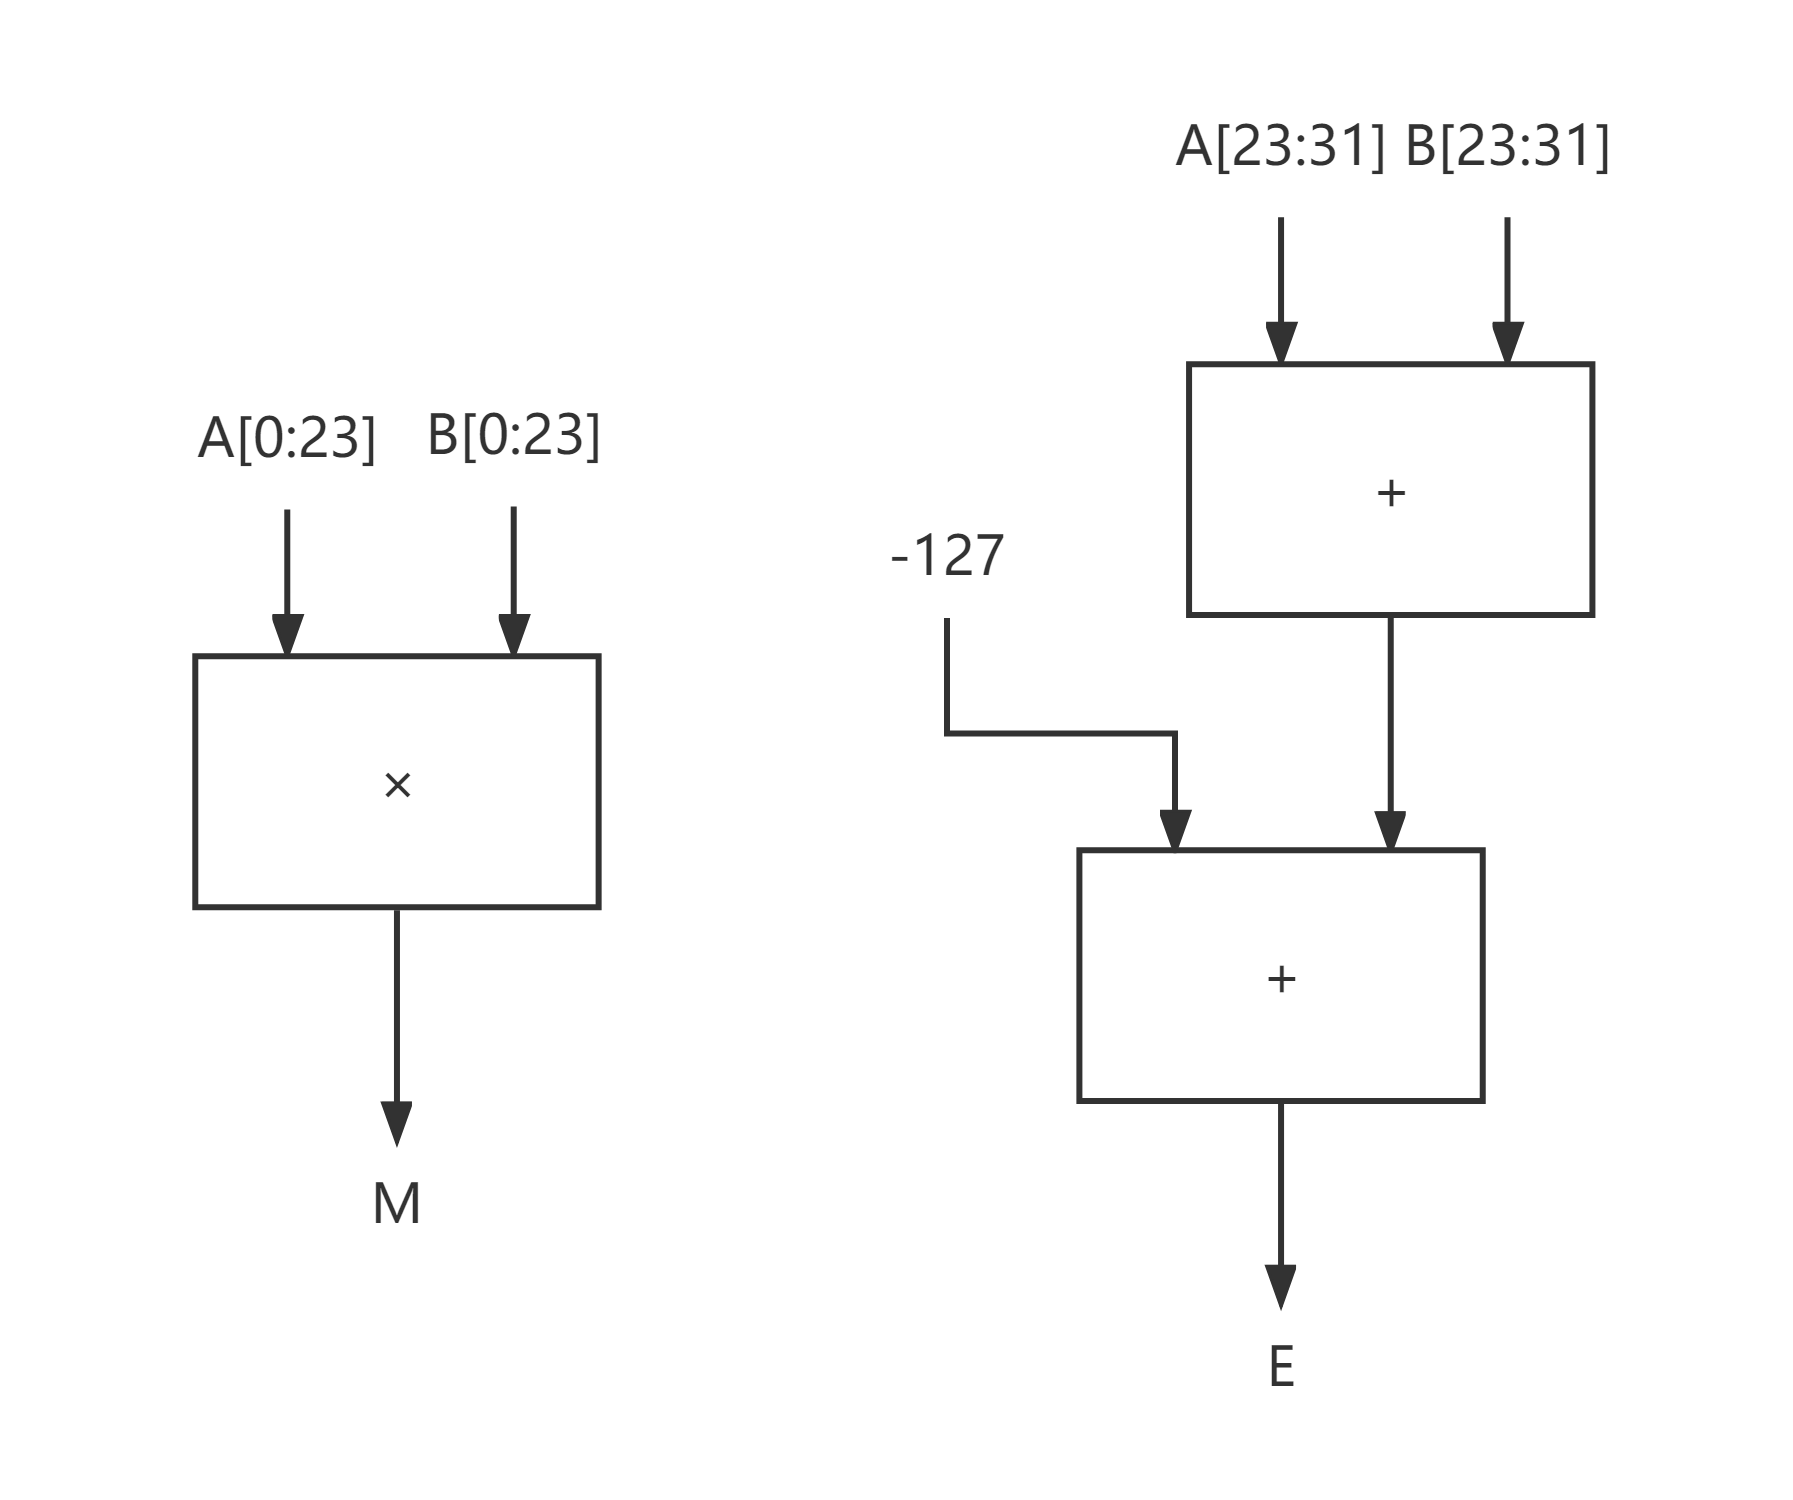
\includegraphics[scale=0.2]{5.png}
\end{figure}
\end{document}
